\documentclass{article}
\usepackage{graphicx} % Required for inserting images
\usepackage{tikz}

\title{Physik - Zusammenfassung fürs Abitur}
\author{Maximilian Penke, Emil Maihorn}
\date{January 2024}

\renewcommand*\contentsname{Gliederung}

\begin{document}

    \maketitle

    \begin{abstract}
        Dies ist eine Zusammenfassung für die Inhalte des Berliner Abiturs von 2024 im Fach Physik. Dabei ist des in die vier Halbjahre unterteilt, wobei es jeweils Differenzierungen gibt. Dafür werden die Inhalte der Einzelthemen erklärt, mit der allgemeinen Umsetzungsweise versehen und darauf folgend mit unterschiedlichen Beispielen veranschaulicht.
    \end{abstract}

    \tableofcontents

    \section{Allgemeine Hinweise zur Notation}

        \subsection{Koordinatensysteme} 

        
        Zu beachten:
        \begin{itemize}
            \item Die Pfeile an der x- und y-Achse und die x- und y- Achsenbeschriftung
            \item Die Kennzeichnung des Koordinatenursprungs und die x- und y-Achseneinteilung
            \item Die Einzeichnung eines Punktes mit einem Kreuz
            \item Punktkennzeichnung mit der Beschreibung
        \end{itemize}

        \begin{figure}[h]
            \centering
            \begin{tikzpicture}[x=1cm, y=1cm]
                % Axes
                \draw [->] (0,0) -- (3,0) node [right] {x [Physikalische Einheit] };
                \draw [->] (0,0) -- (0,3) node [left] {y [Physikalische Einheit]};
                \draw [-] (0,0) -- (-3,0) node [right] {};
                \draw [-] (0,0) -- (0,-3) node [left] {};
            
                \draw [-] (-0.1, -0.1) -- (0.1,0.1);
                \node [below] at (-0.2,0) {0};
                \draw [-] (1, -0.1) -- (1,0.1);
                \node [below] at (1,-0.1) {1};
                \draw [-] (-0.1, 1) -- (0.1,1);
                \node [left] at (-0.2,1) {1};
                \draw [-] (1.5, 1.4) -- (1.4,1.5);
                \draw [-] (1.4, 1.4) -- (1.5,1.5);
                \node [above] at (1.5,1.5) {$P(1.45|1.45)$};
            \end{tikzpicture}
        \end{figure}

        Beispiel:

        \begin{figure}[h]
        \centering
        \begin{tikzpicture}[x=1cm, y=1cm]
            % Axes
            \draw [->] (0,0) -- (3,0) node [right] {t [s] };
            \draw [->] (0,0) -- (0,3) node [left] {U [V]};
            \draw [-] (0,0) -- (-3,0) node [right] {};
            \draw [-] (0,0) -- (0,-3) node [left] {};
        
            \draw [-] (-0.1, -0.1) -- (0.1,0.1);
            \node [below] at (-0.2,0) {0};
            \draw [-] (1, -0.1) -- (1,0.1);
            \node [below] at (1,-0.1) {1};
            \draw [-] (-0.1, 1) -- (0.1,1);
            \node [left] at (-0.2,1) {1};
            \draw [-] (1.5, 1.4) -- (1.4,1.5);
            \draw [-] (1.4, 1.4) -- (1.5,1.5);
            \node [above] at (1.5,1.5) {$P(1.45s|1.45V)$};
        \end{tikzpicture}
    \end{figure}
        
        \subsection{Felder skizzieren}
        
            Zu beachten:
            \begin{enumerate}
                \item Vektoren sind Pfeile
                \item Der Schwanz eines Vektors beginnt stets am Ursprung
                \item Der Kopf eines Vektors endet stets 
            \end{enumerate}

        \subsection{Schaltkreise und Versuchsaufbauten}

        \subsection{Notation in der Rechnung}

            Geg, Ges und Lös sind nicht Pflicht aber hilfreich! \\
            Einheitenumrechnung ist ebenfalls nicht Pflicht, aber eine sehr gute Methode, um die Korrektheit der Antwort zu überprüfen. Diese kann in einer Nebenrechnung vollzogen werden. \\
            Generell gilt: stets in 10er-Potenzen umformen und damit rechnen! \\
            Regeln zur Potenzumformung: $10^m \cdot 10^n = 10^{m+n}$, $\frac{10^m}{m^n} = 10^{m-n}$ \\
            Stets bedenken: Aus Subtraktionen und Summen kürzen nur die Dummen! \\

    \section{Q1: Felder}

        \subsection{Einführung in Felder}
            In der Physik werden Felder genutzt, um Kräfte, Flüsse und Bewegungen zu beschreiben.
            Die Felder, die für uns wichtig sind, sind sog. Vektorfelder der Elektromagnetischen Kraft
            und der Gravitationskraft. \\
            In der Physik werden Kräfte zwischen zwei Objekten gerne mit Vektoren beschrieben. Ungefähr so:
            \begin{figure}[h]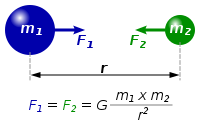
\includegraphics{graphics/universalGravitation.png}\end{figure}          
        \subsection{Darstellung von Feldern}

            

        \subsection{Gravitationsfelder und Astronomie}

            \subsubsection{Keplersche Gesetze}

            \subsection{Gravitationskraft und Berechnung}

            \subsubsection{Gravitationsfeld}

        \subsection{Elektrische Felder und Kondensatoren}

    \section{Q2: Elektromagnetische Wellen}

    \section{Q3: Quantenphysik}

    \section{Q4: Kernphysik}
\end{document}




